

\documentclass[12pt,a4paper]{article}
\usepackage{graphicx}
\usepackage{etex,datetime,setspace,latexsym,amssymb,amsmath,amsthm}
\usepackage{fancybox,dialogue,float,wrapfig,enumerate,microtype}
\usepackage{verbatim,xcolor,multicol,titlesec,tabularx,mdframed}

\usepackage[utf8]{inputenc}
\usepackage[pdftex]{hyperref}
\usepackage[margin=2cm,bottom=3cm,footskip=15mm]{geometry}
\parindent0cm
\parskip0.5em

\usepackage{mathtools}
\usepackage{graphicx}

% 定义一个新的“反向 models”符号
\newcommand{\leftmodels}{\mathrel{\reflectbox{$\models$}}}
% 定义 split disjunction 符号(向右旋转 90°)
\newcommand{\inqdisj}{\mathrel{\raisebox{1.5ex}{\rotatebox{-90}{$\geqslant$}}}}

\usepackage{tikz}
\usetikzlibrary{arrows,trees,positioning,shapes,patterns}
\usetikzlibrary{intersections,calc,fpu,decorations.pathreplacing}

\usepackage[T1]{fontenc} % better fonts

% Haskell code listings in our own style
\usepackage{listings,color}
\definecolor{lightgrey}{gray}{0.35}
\definecolor{darkgrey}{gray}{0.20}
\definecolor{lightestyellow}{rgb}{1,1,0.92}
\definecolor{dkgreen}{rgb}{0,.2,0}
\definecolor{dkblue}{rgb}{0,0,.2}
\definecolor{dkyellow}{cmyk}{0,0,.7,.5}
\definecolor{lightgrey}{gray}{0.4}
\definecolor{gray}{gray}{0.50}
\lstset{
  language        = Haskell,
  basicstyle      = \scriptsize\ttfamily,
  keywordstyle    = \color{dkblue},     stringstyle     = \color{red},
  identifierstyle = \color{dkgreen},    commentstyle    = \color{gray},
  showspaces      = false,              showstringspaces= false,
  rulecolor       = \color{gray},       showtabs        = false,
  tabsize         = 8,                  breaklines      = true,
  xleftmargin     = 8pt,                xrightmargin    = 8pt,
  frame           = single,             stepnumber      = 1,
  aboveskip       = 2pt plus 1pt,
  belowskip       = 8pt plus 3pt
}
\lstnewenvironment{code}[0]{}{}

% only shown, not compiled:
\lstnewenvironment{showCode}[0]{\lstset{numbers=none}}{}

% only compiled, not shown:
\newcommand{\hide}[1]{}

% will the real phi please stand up
\renewcommand{\phi}{\varphi}

% load hyperref as late as possible for compatibility
\usepackage[pdftex]{hyperref}
\hypersetup{
  pdfborder = {0 0 0},
  breaklinks = true,
  linktoc = all,
}
\pdfinfoomitdate=1
\pdftrailerid{}
\pdfsuppressptexinfo15


\title{A Haskell-based Model Checker for Bilateral State-based Modal Logic (BSML)}
\author{Yuan Ma \and Simon Chiu \and Siyuan Wu \and Hangjian Chen \and Hongqian Xia}
\date{\today}
\hypersetup{pdfauthor={Group 2}, pdftitle={A Model Checker for Bilateral State-based Modal Logic (BSML)}}

\begin{document}

\maketitle

\begin{abstract}

    Bilateral State-based Modal Logic (BSML), proposed by \citet{Aloni2024}, 
    extends classical modal logic by adopting state-based semantics and introducing a non-emptiness atom to account for free choice inferences in natural language. 
    This project focuses on developing a Haskell-based model checker for BSML.\@  
    We begin with a breif introduction to the motivation and semantics of the framework, followed by a discussion of its implementation in Haskell.\@ 
    Additionally, we use QuickCheck to verify several key properties about BSML.\@ 
    Finally, we present a web interface that allows users to interact with the model checker and explore BSML.\@

\end{abstract}


\tableofcontents

\clearpage

% We include one file for each section. The ones containing code should
% be called something.lhs and also mentioned in the .cabal file.


\section{Introduction}\label{sec:Introduction}

Haskell, as a functional programming language, 
emphasizes purity (no side effects) and immutability (no data modification). 
This makes Haskell particularly well-suited for handling logical systems, 
as it provides a clean and efficient way to model and manipulate abstract structures. 

BSML is a non-classical modal logic system within formal semantics. This project implements a model checker in Haskell, 
using QuickCheck to verify the reliability of the implementation. 
Additionally, a webpage interface has been created to facilitate user interaction. 

Chapter 2 introduces the linguistic background and motivation behind BSML, along with the system's key non-classical aspects. 
Chapter 3-4 delves into the syntax and semantics of BSML, as well as the Haskell implementation, which forms the core of the model checker. 
Chapter 5 introduces QuickCheck. 
Finally, Chapter 6 explains the web implementation and provides practical usage examples.

\section{Motivation}\label{Motivation}

BSML (Bilateral State-Based Modal Logic) originates from a project led by Maria, 
titled \textit{N∅thing is Logical} (NihiL)\footnote{For details, see \url{https://www.marialoni.org/Nihil}.}. 
This project concerns formal semantics, which employs formalized methods—such as logic and mathematics—to analyze linguistic meaning. 
Natural language does not always conform to classical logic. Consequently, formal semanticists develop non-classical logical systems to better capture linguistic phenomena.

BSML was initially designed to address a well-known issue in linguistics: free choice. Consider the following sentence:

\begin{quote}
    You may go to the beach or to the cinema.
\end{quote}

In natural language, this typically allows the inference:

\begin{quote}
    You may go to the beach, and you may go to the cinema.
\end{quote}

However, in classical modal logic, this inference does not hold. Specifically, from $\Diamond (a \vee b)$, we cannot derive $\Diamond a \land \Diamond b$.

A common strategy in semantics is to attribute certain inferences to pragmatics. 
That is, while semantics concerns literal meaning, pragmatics examines how meaning is shaped by context. For instance, if one says:

\begin{quote}
    Some students in this class are studying logic.
\end{quote}

listeners typically infer that not all students are studying logic——otherwise, the speaker would have simply stated, ``All students are studying logic''.
This inference is not a semantic entailment but rather a pragmatic inference.
In the case of free choice, the inference from disjunction to conjunction is also attributed to pragmatics.

Maria's approach to free choice is based on the idea that speakers construct mental models of reality when interpreting sentences. Her central claim (see \citet{Aloni2022}), termed \textbf{Neglect-Zero}, is as follows
\begin{quote}
    \textbf{Neglect-Zero:} 
     When interpreting a sentence, speakers construct mental models of reality.In doing so, they systematically neglect structures that satisfy the sentence through an empty configuration (zero-models).
    
\end{quote}
Intuitively, this means that when interpreting a disjunction, speakers ignore the possibility of an empty disjunct. For example, in the sentence ``Some boxes are black'', speakers typically do not consider the possibility of an empty box.


BSML formalizes this tendency by introducing the \textit{nonemptiness atom} (NE), which ensures that only nonempty states are considered in the interpretation of sentences. 
This leads to the prediction of both narrow-scope and wide-scope FC inferences, as well as their cancellation under negation.

BSML is built upon team semantics, meaning that formulas are evaluated with respect to sets of possible worlds (teams) rather than individual worlds. 
For example, in Figure\ref{fig.disjunct}, the black small square represents a state in a universe. $\(b\)$ is the zero-model of \( a \vee b \), because one of the disjuncts is empty.

\begin{figure}[h]
    \centering
    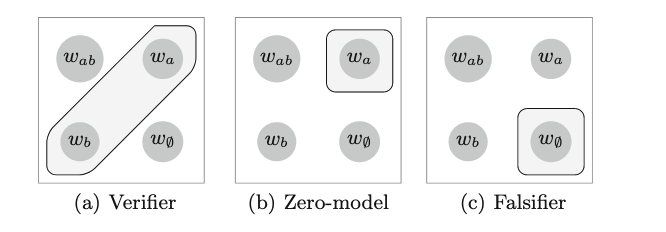
\includegraphics[width=\textwidth]{image/disj1.png}
    \caption{Models for \( a \vee b \)}
    \label{fig.disjunct}
\end{figure}

Additionallt, BSML relies on a bilateral semantics, where each formula has both \textbf{support/assertion conditions ($\models$)} and \textbf{anti-support/rejection conditions ($\leftmodels$)}.

\begin{quote}
    $M, s \models \varphi$: \( \varphi \) is assertable in information state \( s \), with \( s \subseteq W \).

    $M, s \leftmodels \varphi$: $\varphi$ is rejectable in information state $s$, with $s \subseteq W$.
\end{quote}

And logical consequence is defined as preservation of support. 

\begin{quote}
\(\varphi \models \psi\) \quad \text{iff} \quad $\forall M, s : M, s \models \varphi \Rightarrow M, s \models \psi$
\end{quote}


The pragmatic enrichment function \({[ \varphi ]}^+\) modifies the interpretation of formulas:

\begin{quote}
For any formula \( \varphi \): s \models $[\varphi]^+$ \quad \text{iff} \quad s \models \varphi \text{ and } s \neq \emptyset.
\end{quote}

 Based on team-seamantics, BSML adopts a split disjunction based on state-based semantics:

\begin{quote}
    $M, s \models \varphi \vee \psi \colon \Leftrightarrow$ there exist $t, u$ such that $s = t \cup u$ and $M, t \models \varphi$ and $M, u \models \psi$.
    
    $M, s \leftmodels \varphi \vee \psi \colon \Leftrightarrow M, s \leftmodels \varphi$ and $M, s \leftmodels \psi$.
\end{quote}


BSML can be extended with global disjunction:
\begin{itemize}
    \item \(\textbf{BSML}^{\inqdisj}\): This extension adds the \textit{global disjunction} \(\inqdisj\), which allows for the expression of properties that are invariant under bounded bisimulation.
\end{itemize}

The global disjunction also called inquisitive disjunction. 
Inquisitive semantics commonly employs a global disjunction to capture questions. 


With these approach, we establish a robust logical framework capable of predicting linguistic phenomena. 
By comparing these predictions with actual language usage in the real world, we can gain valuable insights into the underlying mechanisms of language.
It is easy to see that pragmatic enrichment has a non-trivial effect on disjunctions, 
and it has non-trivial effects only on disjunctions and only if they occur in a positive environment.  

\begin{itemize}
    \item \textbf{Narrow Scope FC:} \quad ${[ \Diamond (\alpha \lor \beta) ]}^+ \models \Diamond \alpha \land \Diamond \beta$
    \item \textbf{Wide Scope FC:} \quad ${[\Diamond \alpha \lor \Diamond \beta]}^+ \models \Diamond \alpha \land \Diamond \beta$ 
          \quad (if $R$ is indisputable)
    \item \textbf{Dual Prohibition:} \quad ${[\neg \Diamond (\alpha \lor \beta)]}^+ \models \neg \Diamond \alpha \land \neg \Diamond \beta$
    \item \textbf{Double Negation:} \quad ${[\neg \neg \Diamond (\alpha \lor \beta)]}^+ \models \Diamond \alpha \land \Diamond \beta$
 \end{itemize}
 
 This project adopts $BSML^{\inqdisj}$, and the following is the specific Haskell implementation.
   

\input{lib/Syntax.lhs}

\input{lib/Semantics.lhs}

\input{test/simpletests.lhs}


\input{lib/Parser.lhs}
\input{exec/Main.lhs}

\section{Conclusion}\label{sec:Conclusion}

In this project, we have developed a Haskell-based model checker for BSML (Bilateral State-Based Modal Logic). 
We first provided a concise introduction to the core framework of BSML and its extension with global disjunction.
We then implemented its models, syntax, and semantics in Haskell, ensuring a formal and structured representation of the system.\@ 
To validate our implementation, we used QuickCheck to verify several key properties of BSML.\@
Additionally, we developed a web interface to make the model checker more accessible and user-friendly.
BSML offers a robust framework for capturing free-choice inferences in natural language,
and our Haskell-based implementation provides an efficient and reliable tool for analyzing complex models and formulas.


Currently, our implementation of BSML is restricted to natural deduction, and Haskell does not yet provide a way to handle assumptions within this framework.
Future work could focus on developing a sequent calculus for BSML, which would enable a more expressive proof system within the framework.
This would allow for a more comprehensive exploration of the logical properties of BSML and its applications in natural language semantics.

Additionally, BSML has many other extended versions, all of which could be implemented in Haskell in the future, such as:

\textbf{QBSML} (see \cite{Aloni2023}) extends BSML with quantification over possible worlds and states. Implementing this extension in Haskell would refine our model checker to handle richer linguistic sentences, thus enhancing the expressiveness of BSML.\@

\textbf{Bilateral Update Semantics (BiUS)} (See \cite{BiUS2023}) introduces a dynamic perspective on meaning change, incorporating updates. Implementing BiUS in the current model checker could enhance its ability to model information dynamics in discourse.

These extensions will improve the expressiveness of BSML and further demonstrate Haskell's suitability for formal semantic modeling.

In conclusion, our Haskell-based model checker for BSML provides a solid foundation for exploring the logical properties of natural language semantics.
The combination of Haskell's strong type system and functional programming paradigm with the expressive power of BSML offers a promising avenue for future research in this field.



\addcontentsline{toc}{section}{Bibliography}
\bibliographystyle{plainnat}
\bibliography{references.bib}

\end{document}
